\documentclass{cygclanek}
\addbibresource{example_ref.bib}
\begin{document}

\title{Návod k šabloně}

\names{
    \name[*]{Matěj Rzehulka}{fjfi}, \name{Jára Cimrman}{nerc,abc}, \name{Bilbo Baggins}{fvu,nerc}, \name{Frodo Baggins}{nerc}
}
\institutions{
    \institution{fvu}{Fiktivní výzkumný ústav, Neexistující ulice 5, 999 99 Nikde, ČR}
    \institution{nerc}{Non-existing research centre, 5.25 New street, SM PSTCD, Some Country}
    \institution{abc}{Somewhere}
    \institution{fjfi}{FJFI ČVUT v Praze, Břehová 7, 115 19 Praha 1, ČR}
}

\email{rzehumat@fjfi.cvut.cz}
\year{2022}

\maketitle
\begin{abstract}
    Abstrakt napište mezi \verb|\begin{abstract}| a \verb|\end{abstract}|.
\end{abstract}
\keywords{Klíčová slova napište do tagu keywords.}

\section{Úvod}

Tento dokument slouží jako návod. 

\section{Teorie}
Tady demonstrujeme několik možností, jak tuto šablonu používat.

\subsection{Izotopy, reakce, chemie}
Izotopy lze psát pomocí \verb|\ce|, např. \verb|\ce{^{2}D}| vytvoří \ce{^{2}D}. Podobně to lze použít i na 
reakce - např. \verb|\ce{^{10}B(n,\alpha) ^7Li}| je \ce{^{10}B(n,\alpha) ^7Li}. Alternativně lze 
použít i šipku, což se dá napsat jako\newline\verb|\ce{^{10}B + n -> ^4He + ^7Li}| 
a vytvoří \ce{^{10}B + n -> ^4He + ^7Li}. 

Pomocí \verb|\ce| lze psát i chemické reakce, např.\verb|\ce{H2SO4 + 2NaOH -> Na2SO4 + 2H2O}| vytvoří \ce{H2SO4 + 2NaOH -> Na2SO4 + 2H2O}.

    Prostředí \verb|\ce| je \uv{univerzální}, lze jej používat jak v textu, tak i v matematickém módu 
    (tj. části vymezené \verb|{$...$}|, \verb|$$ ... $$|, \verb|\begin{equation}...\end{equation}| atd.

Prostředí \verb|\ce| pochází z balíčku \verb|mhchem| \cite{ctan_mhchem} (není třeba nic přidávat 
pomocí \verb|\usepackage|, balíček už je zahrnut v~\verb|documentclass|).

\subsection{Čísla, jednotky}
Čísla se mohou normálně psát do textu, jako 2, 3, 314,579 atd. To však má několik 
problémů - mezera mezi tisícemi se nedělá automaticky, desetinnou tečku/čárku nelze hromadně měnit, 
zápis nejistot je velmi pracný, atd.

Lepší je používat příkaz \verb|\num| z balíčku \verb|siunitx| \cite{ctan_siunitx} (už přidáno 
v rámci šablony). Např. \verb|\num{5672684}|, \verb|\num{3.25e6}|, \verb|\num{2.25(1)e6}| vytvoří 
\num{5672684}, \num{3.25e6}, \num{2.25(1)e6}. Pro dlouhý zápis chyby pak lze použít 
\verb|\num[separate-uncertainty=true]{2.25(1)e6}|, což vytvoří \num[separate-uncertainty=true]{2.25(1)e6}.

    Správné psaní jednotek lze psát příkazem \verb|\si|. Funguje běžně v textu i v matematickém módu, takže 
    elegantně řeší problém s nežádoucí kurzívou u jednotek. Např. \verb|\si{cm^3}| vytvoří \si{cm^3}. 
    Zápis akceptuje lomítka nebo násobení (pomocí \verb|\cdot| lze vytvořit znak $\cdot$), mocniny, řečtinu atd. 
    Speciální problém pak je předpona \uv{mikro}, kde je potřeba stojatého $\mu$ -- toho se docílí pomocí 
    \verb|\micro|, např.~\verb|\si{\micro m}| vytvoří \si{\micro m}. 

    Častým problémem je psaní stupňů -- to lze pomocí \verb|\ang{68}|, \ang{68}. Stupně Celsia pak lze psát 
    jako jednotku \verb|\si{\celsius}| \si{\celsius}.


Vhodnou mezeru mezi číslem a jednotkou a kombinaci \verb|\num| a \verb|\si| je \verb|\SI|, použitelné např.
    jako \verb|\SI{5.236}{MeV}|, \SI{5.236}{MeV} nebo \verb|\SI{5.236(1)}{\micro eV}|, \SI{5.236(1)}{\micro eV}. 
    Funckcionalita je stejná v textu i v matematickém módu.


\subsection{Rovnice a symboly}
    Nejlepší nástroj k nalezení symbolů v (La)\TeX u je Detexify \cite{detexify}.

Rovnice a symboly používané v rovnicích lze psát do řádku jako \verb|$a = b$| $a = b$. 

Pro zápis přes celou šířku včetně reference lze použít prostředí equation
    \begin{lstlisting}[language=TeX]
        \begin{equation}
          D\nabla^2\phi - \Sigma_a\phi + \nu\Sigma_f\phi = \frac{1}{v}
            \frac{\partial\phi}{\partial t}\,.
          \label{difuzka}
        \end{equation}
    \end{lstlisting}
    vytvoří 
\begin{equation}
  D\nabla^2\phi - \Sigma_a\phi + \nu\Sigma_f\phi = \frac{1}{v}\frac{\partial
  \phi}{\partial t}\,.
  \label{difuzka}
\end{equation}

Více rovnic pod sebou se zarovnáním lze vytvořit v prostředí \verb|align|
\begin{lstlisting}[language=TeX]
\begin{align}
  a &= b \label{rovnice_a} \,,\\
  b &= c \label{rovnice_b} \,.
\end{align}
\end{lstlisting}
vytvoří
\begin{align}
  a &= b \label{rovnice_a} \,,\\
  b &= c \label{rovnice_b} \,.
\end{align}


\subsection{Tabulky}

Dobrý návod je na Overleafu \cite{overleaf_tables}. Dva příklady jsou pak níže. Písmeno v hranaté závorce 
je pozice. \verb|H| znamená, že tabulka bude přesně na tom místě, kde je v kódu - což může, ale ne vždy 
vypadá dobře. Naproti tomu \verb|h| se snaží dát tabulku tam, kde je v kódu, ale zachovává jistou flexibilitu 
a snaží se dát tabulku tak, aby výsledek vypadal dobře.

\begin{verbatim}
    \begin{table}[H]
    \centering
    \caption{Tabulka -- návrh tzv. \uv{čistá}.}
    \label{mer}
    \begin{tabular}{ccc}
    	\toprule
    $\rho$ [\textcent] & $T_e$ [s] & $T_d$ [s] \\
    \midrule
    \num{3.6} &  \num{312.95(1)} & \num{216.92(1)} \\
    \num{6.5} &  \num{162.22(2)} & \num{112.44(1)} \\
    \num{9.8} &  \num{96.79(9)}  & \num{67.61(6)} \\
    \num{12.8} & \num{68.06(2)}  & \num{47.18(1)} \\
    \num{15.5} & \num{51.36(6)}  & \num{35.60(4)} \\
    \num{19.0} & \num{38.11(4)}  & \num{26.47(3)} \\
    \bottomrule
    \end{tabular}
    \end{table}
\end{verbatim}

    \begin{table}[H]
    \centering
    \caption{Tabulka -- návrh tzv. \uv{čistá}.}
    \label{mer}
    \begin{tabular}{ccc}
    	\toprule
    $\rho$ [\textcent] & $T_e$ [s] & $T\_d$ [s] \\
    \midrule
    \num{3.6} &  \num{312.95(1)} & \num{216.92(1)} \\
    \num{6.5} &  \num{162.22(2)} & \num{112.44(1)} \\
    \num{9.8} &  \num{96.79(9)}  & \num{67.61(6)} \\
    \num{12.8} & \num{68.06(2)}  & \num{47.18(1)} \\
    \num{15.5} & \num{51.36(6)}  & \num{35.60(4)} \\
    \num{19.0} & \num{38.11(4)}  & \num{26.47(3)} \\
    \bottomrule
    \end{tabular}
    \end{table}

\begin{verbatim}
\begin{table}[H]
    \centering
    \caption{Tabulka \uv{plná}.}
    \label{ver}
    \begin{tabular}{|c|c|c|}
        \hline
        $\rho$ [\textcent] & $T_e$ [s] & $T\_d$ [s] \\
        \hline
        \num{3.6} &  \num{312.95(1)} & \num{216.92(1)} \\
        \hline
        \num{6.5} &  \num{162.22(2)} & \num{112.44(1)} \\
        \hline
        \num{9.8} &  \num{96.79(9)}  & \num{67.61(6)} \\
        \hline
        \num{12.8} & \num{68.06(2)}  & \num{47.18(1)} \\
        \hline
        \num{15.5} & \num{51.36(6)}  & \num{35.60(4)} \\
        \hline
        \num{19.0} & \num{38.11(4)}  & \num{26.47(3)} \\
        \hline
    \end{tabular}
\end{table}
\end{verbatim}

\begin{table}[H]
    \centering
    \caption{Tabulka \uv{plná}.}
    \label{ver}
    \begin{tabular}{|c|c|c|}
        \hline
        $\rho$ [\textcent] & $T_e$ [s] & $T\_d$ [s] \\
        \hline
        \num{3.6} &  \num{312.95(1)} & \num{216.92(1)} \\
        \hline
        \num{6.5} &  \num{162.22(2)} & \num{112.44(1)} \\
        \hline
        \num{9.8} &  \num{96.79(9)}  & \num{67.61(6)} \\
        \hline
        \num{12.8} & \num{68.06(2)}  & \num{47.18(1)} \\
        \hline
        \num{15.5} & \num{51.36(6)}  & \num{35.60(4)} \\
        \hline
        \num{19.0} & \num{38.11(4)}  & \num{26.47(3)} \\
        \hline
    \end{tabular}
\end{table}


% \subsection{Obrázky}
% Relevantní tutoriály: \cite{overleaf_thesis3,overleaf_images,overleaf_positioning}. Syntax je podobná jako 
% u tabulek.
% 
% Je třeba poskytnout buďto relativní cestu k souboru obrázku nebo, je-li obrázek ve složce \verb|img|, stačí 
% název.
% 
% \begin{verbatim}
% \begin{figure}[h]
%     \centering
%     
\includegraphics[width=0.4\textwidth]{fjfi.pdf}
%     \caption{Ukázkový obrázek.}
%     \label{fig:fjfi_logo}
% \end{figure}
% \end{verbatim}
% 
% \begin{figure}[h]
%     \centering
%     
\includegraphics[width=0.4\textwidth]{fjfi.pdf}
%     \caption{Ukázkový obrázek.}
%     \label{fig:fjfi_logo}
% \end{figure}
% 
% Alternativně (jelikož syntax výše je poměrně zdlouhavá), lze použít zkrácenou verzi.
% \begin{verbatim}
% \obr{fjfi.pdf}{Nejaky obrazek bez nepovinneho \uv{parametru}. Vypada trochu moc
% velky.}{fig:moc-velky-obrazek}[0.4]
% \end{verbatim}
% 
% \obr{fjfi.pdf}{Nejaky obrazek bez nepovinneho \uv{parametru}. Vypada trochu moc
% velky.}{fig:moc-velky-obrazek}[0.4]
% 
% Název \uv{Obrázek} se ne vždy hodí. Název se dá změnit pomocí \verb|\captionsetup{name=...}|, např.
% 
% \begin{verbatim}
% \begin{figure}[h]
%     \centering
%     \captionsetup{name=Graf}
%     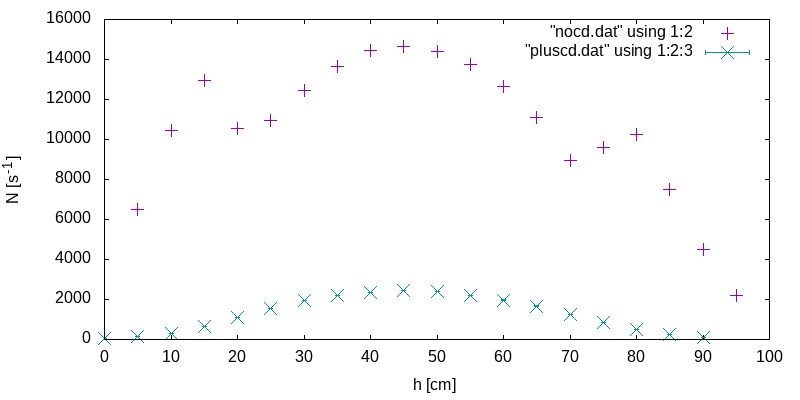
\includegraphics[width=0.4\textwidth]{both.png}
%     \caption{Nějaký graf.}
%     \label{fig:graf}
% \end{figure}
% \end{verbatim}
% 
% \begin{figure}[h]
%     \centering
%     \captionsetup{name=Graf}
%     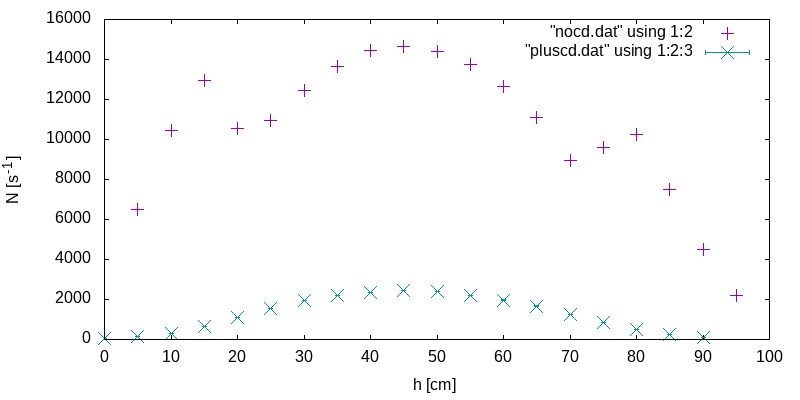
\includegraphics[width=0.4\textwidth]{both.png}
%     \caption{Nějaký graf.}
%     \label{fig:graf}
% \end{figure}
% 
% Zkrácená verze pak je \verb|\graf{both.png}{Nejaky graf.}{fig:takygraf}|.
% \graf{both.png}{Nejaky graf.}{fig:takygraf}
% 
% Je-li potřeba dát dva obrázky vedle sebe, lze použít \verb|minipage|.
% \begin{verbatim}
%     \begin{figure}[H]
%         \centering
%         \begin{minipage}{0.49\textwidth}
%             \centering
%             
\includegraphics[width=0.98\textwidth]{fjfi.pdf}
%             \caption{Levý obrázek.}
%             \label{fig:levy}
%         \end{minipage}\hfill
%         \begin{minipage}{0.49\textwidth}
%             \centering
%             
\includegraphics[width=0.98\textwidth]{symbol_cvut_konturova_verze_cb.pdf}
%             \caption{Pravý obrázek.}
%             \label{fig:pravy}
%         \end{minipage}
%     \end{figure}
% \end{verbatim}
% 
% \begin{figure}[H]
%     \centering
%     \begin{minipage}{0.49\textwidth}
%         \centering
%         
\includegraphics[width=0.98\textwidth]{fjfi.pdf}
%         \caption{Levý obrázek.}
%         \label{fig:levy}
%     \end{minipage}\hfill
%     \begin{minipage}{0.49\textwidth}
%         \centering
%         
\includegraphics[width=0.98\textwidth]{symbol_cvut_konturova_verze_cb.pdf}
%         \caption{Pravý obrázek.}
%         \label{fig:pravy}
%     \end{minipage}
% \end{figure}
% 
% Podobně i zde existují zkrácené verze.
% \begin{verbatim}
% \dobr{fjfi.pdf}{Jeden obrazek. Zřejmě by bylo dobré udělat je stejně velké.
% Proto v~obr.~\ref{fig:srovnany} nastavíme velikost pomocí nepovinneho
% parametru.}{fig:prvni}{symbol_cvut_konturova_verze_cb.pdf}{Druhý obr.}{fig:druhy}
% \end{verbatim}
% 
% \begin{verbatim}
% \dgraf{both.png}{Jeden graf.}{fig:dalsi}{calibration.png}{Druhý graf.}{fig:ddalsi}
% Rozumíte, já po vás nechci žádnou přednášku, jenom ten základní princip a jednu dvě zajímavosti. (Jevištní mistr mlčí.)
% \end{verbatim}


\subsection{Kód}

\subsection{Citace}

\subsection{Odkazy}

\subsection{Indexy}

\subsection{Čeština}











Ke druhé změně \cite{trace_parcs} nás vedla Cimrmanova ručně psaná poznámka na titulním listě hry:
\uv{Nedělat přestávku, jinak utečou.} My tomuto nebezpečí čelíme tím, že
přestávku sice děláme, ale zařazujeme ji hned za třetí obraz hry, což je tak
nečekaně brzy, že se pohádka ani nestačí rozjet. 
\begin{equation}
  D\nabla^2\phi - \Sigma_a\phi + \nu\Sigma_f\phi = \frac{1}{v}\frac{\partial
  \phi}{\partial t}
  \label{difuzka}
\end{equation}

Zde se ozkážeme na rovnici \eqref{difuzka}. 

Podle odhadu našeho psychologa
dr. Pšeničky se publikum o~přestávce rozdělí na dva tábory. Jedni by rádi
odešli domů, ale bude jim prý líto, že vynaložili tolik peněz na tak krátký čas
zábavy. Druzí by také rádi odešli domů, ale ti zase setrvávají ze zvědavosti,
zda bude druhá část představení stejně slabá jako první. A~kromě toho zamykáme
hlavní dveře.


\subsection{Notová osnova}
Ostatně divák, který by si nechal ujít druhou půli večera, by se ošidil
o~výstup v~dějinách inscenační tvorby zcela ojedinělý. Jedná se o~proměnu jedné
osoby v~osobu jinou, která se odehraje přímo před očima diváků, a to podle
vlastního Cimrmanova vynálezu. Tento výjev vzbudil ve své době světový rozruch,
především na Litoměřicku, i byl označován jako \uv{zázrak divadelní techniky.}


\section{Experiment}
Rád bych teď využil té skutečnosti \ref{fig:moc-velky-obrazek}, že má dnes
službu jevištní mistr, který vynález podle Cimrmanova původního nákresu
rekonstruoval, takže by nám o~něm mohl říci několik zajímavostí, zejména
ověření, že 
\begin{align}
  a &= b \label{rovnice_a} \,,\\
  b &= c \label{rovnice_b} \,,
\end{align}

skutečně platí. Na každou z~těch rovnic se můžu odkázat -- třeba takto
\eqref{rovnice_a} a takto \eqref{rovnice_b}.

\dobr{fjfi.pdf}{Jeden obrazek. Zřejmě by bylo dobré udělat je stejně velké.
Proto v~obr.~\ref{fig:srovnany} nastavíme velikost pomocí nepovinneho
parametru.}{fig:prvni}{symbol_cvut_konturova_verze_cb.pdf}{Druhý obr.}{fig:druhy}


\dobr{fjfi.pdf}{Jeden obrazek. Pomocí nepovinných parametrů byla nastavena
šířka.}{fig:srovnany}{symbol_cvut_konturova_verze_cb.pdf}{Druhý
obr.}{fig:jiny}[0.7][0.98]



\subsection{Veselý železničář}
(Zavolá do opony a podrží ji rozevřenou. \uv{Nikdo} se však neobjeví, a tak přednášející zajde za~\ref{fig:prvni} oponu a~\ref{fig:druhy} po chvíli přivede neochotně se tvářícího mistra.)

\graf{both.png}{Nejaky graf.}{fig:takygraf}

Pane kolego, já jsem tu hovořil o~tom Cimrmanově vynálezu, a vy jste ho vlastně rekonstruoval. Buďte tak laskav a povězte divákům, jak to celé funguje. (Mistr mlčí.)

\dgraf{both.png}{Jeden graf.}{fig:dalsi}{calibration.png}{Druhý graf.}{fig:ddalsi}
Rozumíte, já po vás nechci žádnou přednášku, jenom ten základní princip a jednu dvě zajímavosti. (Jevištní mistr mlčí.)

Jevištní mistr: Žádný vodiče tam nejsou. Přednášející: Aha, tak já do toho tak nevidím. Dobře, že vás tu máme. My jenom vidíme, že jak ona tam princezna Zlatovláska stojí, tak se při plném světle uprostřed jeviště promění. Je to tak, nebo ne? (Jevištní mistr přikývne.)

\begin{table}[H]
\centering
\begin{tabular}{|c|c|c|}
\hline
$\rho$ [\textcent] & $T_e$ [s] & $T_d$ [s] \\
\hline
3,6 & $(312,95 \pm 0,01)$ & $(216,92 \pm 0,01)$ \\
\hline
6,5 & $(162,22 \pm 0,02)$ & $(112,44 \pm 0,01)$ \\
\hline
9,8 & $(96,749 \pm 0,009)$ & $(67,061 \pm 0,006)$ \\
\hline
12,8 & $(68,06 \pm 0,02)$ & $(47,18 \pm 0,01)$ \\
\hline
15,5 & $(51,36 \pm 0,06)$ & $(35,60 \pm 0,04)$ \\
\hline
19,0 & $(38,111 \pm 0,004)$ & $(26,417 \pm 0,003)$ \\
\hline
\end{tabular}
\caption{Tabulka \uv{plná}.}
\label{ver}
\end{table}


\section{Závěr}
Že vás ještě přerušuji: já jsem si všiml, že tam je taková soustava vodičů vzájemně propojených, že, která je přesně vyvážená, a celé je to, myslím, pevně fixováno v~portále, ne?
\obr{fjfi.pdf}{Nejaky obrazek s~nepovinnym parametrem sirka = 0.1 strany.}{fig:takapi}[0.1]

Jevištní mistr: Žádný vodiče tam nejsou. Přednášející: Aha, tak já do toho tak nevidím. Dobře, že vás tu máme. My jenom vidíme, že jak ona tam princezna Zlatovláska stojí, tak se při plném světle uprostřed jeviště promění. Je to tak, nebo ne? (Jevištní mistr přikývne.)
\section*{Poděkování}
Přednášející: A~já jsem si právě myslel, že to je způsobeno těmi vodiči, respektive jejich napětím, že se její staré rysy odstraní a nahradí novými. A~to vy ovládáte u~toho řídicího panelu, viďte? Jevištní mistr: Tam sedí Maurenc.



\printbibliography[title={Literatura}]

\end{document}
